\documentclass[fleqn,reqno,10pt]{article}

\usepackage{myarticlestyledefault}

\usepackage{pgfplots}

\begin{document}

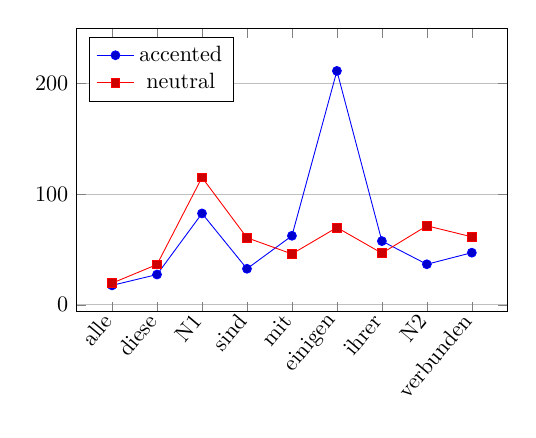
\begin{tikzpicture}[scale=0.8]
  \begin{axis}[
    legend pos = north west,
    ymajorgrids,
    ymax = 250,
    y = 0.5,
    x tick label style = {rotate = 50, anchor = east},
    xtick = data,
    xticklabels = {alle,diese,N1,sind,mit,einigen,ihrer,N2,verbunden}
    ]
    \addplot coordinates {
      (0 ,17.6)
      (1 ,27.4)
      (2 ,82.6)
      (3 ,32.6)
      (4 ,62.4)
      (5 ,211.3333333)
      (6 ,57.6)
      (7 ,36.66666667)
      (8 ,47.13333333)};

  \addplot coordinates {
        (0 ,19.6        )
        (1 ,36.46666667 )
        (2 ,115.1333333 )
        (3 ,60.6        )
        (4 ,46          )
        (5 ,69.86666667 )
        (6 ,46.66666667)
        (7 ,71.4)
        (8 ,61.46666667)};

      \legend{accented, neutral}


  \end{axis}
\end{tikzpicture}


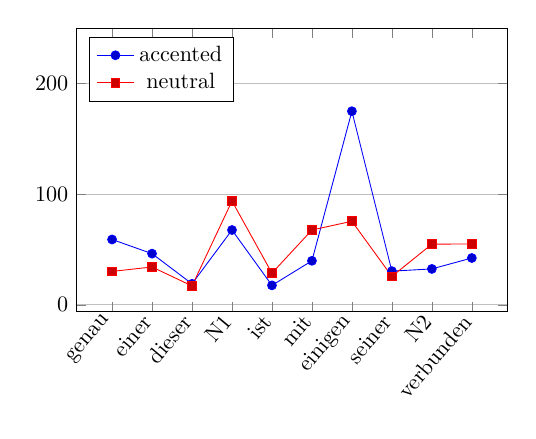
\begin{tikzpicture}[scale=0.8]
  \begin{axis}[
    legend pos = north west,
    ymajorgrids,
    ymax = 250,
    y = 0.5,
    x tick label style = {rotate = 50, anchor = east},
    xtick = data,
    xticklabels = {genau,einer,dieser,N1,ist,mit,einigen,seiner,N2,verbunden}
    ]
    \addplot coordinates {
        (     0 , 59.06666667 )
        (     1 , 46.26666667 )
        (     2 , 19          )
        (     3 , 67.6        )
        (     4 , 17.6        )
        (     5 , 39.8        )
        (     6 , 174.9333333 )
        (     7 , 30.46666667 )
        (     8 , 32.46666667 )
        (     9 , 42.33333333 )};

  \addplot coordinates {
        (0 , 30.21428571 )
        (1 , 34.21428571 )
        (2 , 17.07142857 )
        (3 , 93.78571429 )
        (4 , 28.64285714 )
        (5 , 67.64285714 )
        (6, 75.5        )
        (7 , 25.71428571 )
        (8 , 54.85714286 )
        (9 , 55)};

      \legend{accented, neutral}


  \end{axis}
\end{tikzpicture}

\newpage

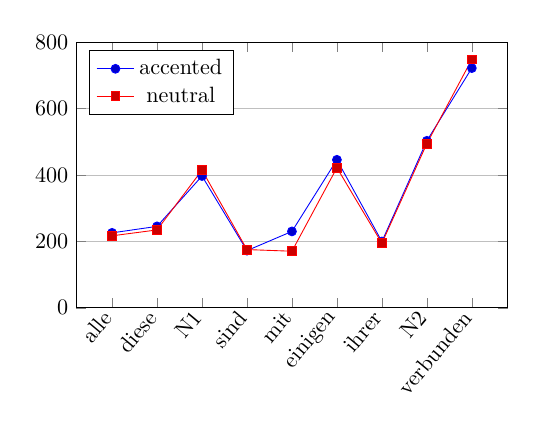
\begin{tikzpicture}[scale=0.8]
  \begin{axis}[
    legend pos = north west,
    ymajorgrids,
    ymax = 800,
    ymin = 0,
    y = 0.15,
    x tick label style = {rotate = 50, anchor = east},
    xtick = data,
    xticklabels = {alle,diese,N1,sind,mit,einigen,ihrer,N2,verbunden}
    ]
    \addplot coordinates {
      (0 ,225.8333333)
      (1 , 245.3333333 )
      (2 , 397         )
      (3 , 172.3333333 )
      (4 , 230.1666667 )
      (5 , 445.8333333 )
      (6, 199.6666667)
      (7, 503)
      (8 ,722 )
    };

  \addplot coordinates {
        (0 , 216.9212    )
        (1 , 234.6666667 )
        (2 , 414.6666667 )
        (3 , 175.5       )
        (4 , 170.5       )
        (5 , 422         )
        (6 , 194.6666667 )
        (7 , 494.6666667 )
        (8 , 748)
};

      \legend{accented, neutral}


  \end{axis}
\end{tikzpicture}

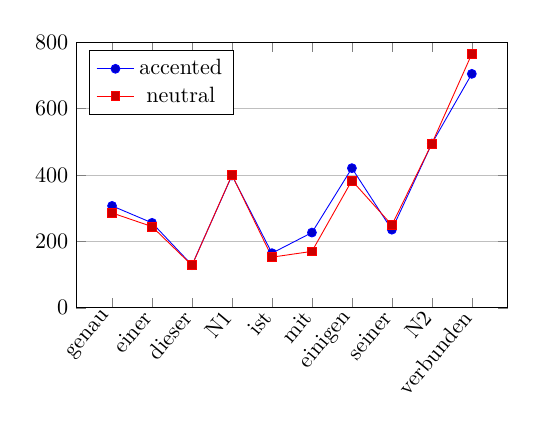
\begin{tikzpicture}[scale=0.8]
  \begin{axis}[
    legend pos = north west,
    ymajorgrids,
    ymax = 800,
    ymin = 0,
    y = 0.15,
    x tick label style = {rotate = 50, anchor = east},
    xtick = data,
    xticklabels = {genau,einer,dieser,N1,ist,mit,einigen,seiner,N2,verbunden}
    ]
    \addplot coordinates {
(       0 , 307         )
(       1 , 256         )
(       2 , 128.6666667 )
(       3 , 398.6666667 )
(       4 , 164.6666667 )
(       5 , 226.6666667 )
(       6 , 420.6666667 )
(       7 , 235.3333333 )
(       8 , 494.6666667 )
(       9 , 704.6666667 )
    };

  \addplot coordinates {
(0 , 285.8333333 )
(1 , 244.6666667 )
(2 , 128         )
(3 , 400         )
(4 , 152.6666667 )
(5 , 170         )
(6 , 383.3333333 )
(7 , 249.3333333 )
(8 , 494.6666667 )
(9 , 764.6666667 )
};

      \legend{accented, neutral}


  \end{axis}
\end{tikzpicture}


\newpage

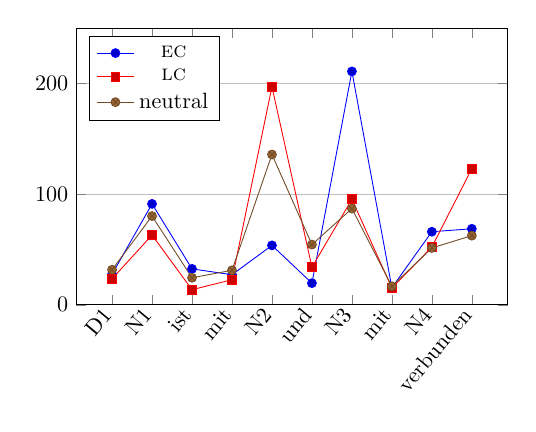
\begin{tikzpicture}[scale=0.8]
  \begin{axis}[
    legend pos = north west,
    ymajorgrids,
    ymax = 250,
    ymin = 0,
    y = 0.5,
    x tick label style = {rotate = 50, anchor = east},
    xtick = data,
    xticklabels = {D1,N1,ist,mit,N2,und,N3,mit,N4,verbunden}
    ]
    \addplot coordinates {
(       0 ,27.65517241 )
(       1 ,91.20689655 )
(       2 ,32.51724138 )
(       3 ,27.20689655 )
(       4 ,53.72413793 )
(       5 ,19.5862069  )
(       6 ,210.8965517 )
(       7 ,15.48275862 )
(       8 ,66.06896552 )
(       9 ,68.72413793 )
    };

  \addplot coordinates {
(0 ,23.48148148) 
(1 ,63.07407407) 
(2 ,13.7037037 ) 
(3 ,22.7037037 ) 
(4 ,197.0740741) 
(5 ,34.03703704) 
(6 ,95.37037037) 
(7 ,15.22222222) 
(8 ,52.18518519) 
(9 ,123        ) };

  \addplot coordinates {
(0, 31.7        )
(1, 80.2        )
(2, 24.46666667 )
(3, 31.2        )
(4, 135.8333333 )
(5, 54.46666667 )
(6, 86.96666667 )
(7, 16.76666667 )
(8, 51.4        )
(9, 62.53333333 )};

      \legend{\textsc{ec},\textsc{lc},neutral}


  \end{axis}
\end{tikzpicture}


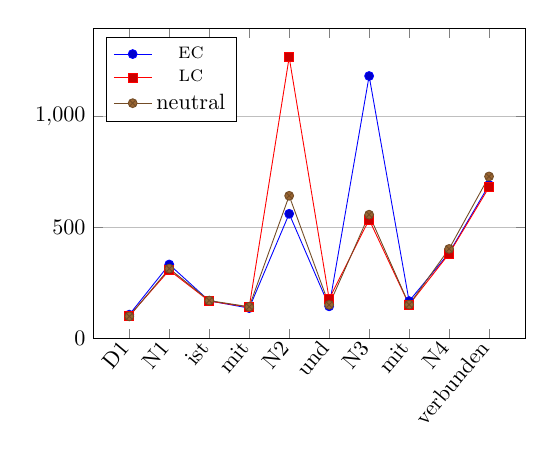
\begin{tikzpicture}[scale=0.8]
  \begin{axis}[
    legend pos = north west,
    ymajorgrids,
    ymax = 1400,
    ymin = 0,
    y = 0.1,
    x tick label style = {rotate = 50, anchor = east},
    xtick = data,
    xticklabels = {D1,N1,ist,mit,N2,und,N3,mit,N4,verbunden}
    ]
    \addplot coordinates {
(0  , 105.75      )
(1  , 332.3333333 )
(2  , 168         )
(3  , 135.3333333 )
(4  , 561.3333333 )
(5  , 143.3333333 )
(6  , 1183.666667 )
(7  , 167         )
(8  , 384.6666667 )
(9  , 691.3333333 )
    };

  \addplot coordinates {
(0  , 100.75      )
(1  , 306.6666667 )
(2  , 167         )
(3  , 139.6666667 )
(4  , 1268.333333 )
(5  , 176.3333333 )
(6  , 535.3333333 )
(7  , 150.3333333 )
(8  , 381         )
(9  , 681.3333333 )
};

  \addplot coordinates {
(0  , 98.08333333 )
(1  , 313.6666667 )
(2  , 169.3333333 )
(3  , 141.3333333 )
(4  , 642.6666667 )
(5  , 150         )
(6  , 557.3333333 )
(7  , 151         )
(8  , 402.6666667 )
(9  , 730)
};

      \legend{\textsc{ec},\textsc{lc},neutral}


  \end{axis}
\end{tikzpicture}


\end{document}
